\documentclass[8pt,a4paper,oneside,hidelinks,aspectratio=169,dvipsnames]{beamer}
\usepackage[outputdir=build]{minted}
\usepackage[T1]{fontenc}
\usepackage[utf8]{inputenc}
\usepackage[english]{babel}
\usepackage{datetime}
\usepackage{lmodern}
\usepackage{graphicx}
\usepackage{csquotes}
\usepackage{amsmath}
\usepackage{caption}
\usepackage{subcaption}
\usepackage{pifont}
\usepackage{xspace}
\usepackage{pgfplots}
\usepackage{tikz}
\usepackage[export]{adjustbox}

\usetheme[progressbar=frametitle]{metropolis}
\setbeamerfont{block title}{size=\small}
\setbeamertemplate{section in toc}[sections numbered]
\captionsetup[figure]{font=tiny,labelsep=none}
\usetikzlibrary{automata, arrows.meta, shapes.geometric, calc, positioning, fit}

\newcommand{\cmark}{\ding{51}\xspace}%
\newcommand{\xmark}{\ding{55}\xspace}%
\newcommand{\code}[1]{\texttt{\detokenize{#1}}}
\newcommand{\codecpp}[1]{\mintinline[fontsize=\small]{C++}{#1}}

\title{Accelerating Halide on an FPGA by using CIRCT and Calyx as an intermediate step to go from a high-level and software-centric IRs down to RTL}
\date{May 15, 2023}
\author{Sergi Granell Escalfet}
\institute[Facultat d’Informàtica de Barcelona] {
  Master Degree in Innovation and Research in Informatics - High Performance Computing \\
  Facultat d’Informàtica de Barcelona \\
  Universitat Politècnica de Catalunya - BarcelonaTech
}

\pgfdeclareimage[height=0.6cm]{university-logo}{img/logo-upc-fib.png}
%\logo{\pgfputat{\pgfxy(-1.4,-1.0)}{\pgfbox[center,base]{\pgfuseimage{university-logo}}}}

\begin{document}

\maketitle

\begin{frame}
  \frametitle{Table of Contents}
  \tableofcontents
\end{frame}

\section{Introduction}

\begin{frame}{Image and array processing}
  \begin{itemize}
    \item Image processing and array processing play an essential role in modern life:
          \begin{itemize}
            \item Applying filters to the images that we upload to social media
            \item Running object detection algorithms on self-driving cars
          \end{itemize}
    \item $\uparrow$ \textbf{Sophistication} modern image processing pipelines, resolution image sensors, real-time video processing $\implies$ $\uparrow$ demand for highly \textbf{efficient} image processing pipeline implementations
    \item \textbf{Diversity} of targets: from a small device such as a smartphone, smartwatch or edge device to large data center and HPC systems
    \item Optimizing these algorithms can be \textbf{complex} and often results in \textbf{non-portable code}
          \begin{itemize}
            \item Hand-tuned C and assembly for a specific architecture
            \item Implementations optimized for an x86 multicore and a modern GPU have little resemblance
          \end{itemize}
  \end{itemize}
\end{frame}

\begin{frame}{Domain Specific Languages (DSLs)}
  \begin{itemize}
    \item DSLs: programming languages specialized to a \textbf{particular application domain}
    \item \textbf{Abstraction}: they provide a higher level of abstraction tailored to the specific domain
          \begin{itemize}
            \item Making it easier for developers to express complex concepts and ideas in a concise and natural way
          \end{itemize}
    \item \textbf{Expressiveness}: by focusing on a specific domain, DSLs enable developers to express their intent more directly, resulting in more readable and maintainable code
    \item \textbf{Productivity}: they simplify the development process. Focus on solving domain-specific problems rather than low-level implementation details
    \item \textbf{Performance}: they can be optimized for the specific domain, potentially allowing more efficient execution and better performance
    \item For the image/array processing application domain $\implies$ \textbf{Halide}
  \end{itemize}
\end{frame}

\section{Halide}

\begin{frame}[fragile]{Halide}
  \begin{itemize}
    \item Main idea: \textbf{decouple} the \textcolor{blue}{\textbf{\textit{algorithm}}} (\textquote{what needs to be computed}) definition from its \textcolor{blue}{\textbf{\textit{schedule}}} (\textquote{how it should be computed})
    \item W/o changing algorithm, explore different optimizations strategies (loop nesting and loop fusion, tiling, recomputation and storage balancing, vectorization, parallelism, \ldots)
  \end{itemize}
  \begin{figure}[H]
    \centering
    \begin{minipage}{\textwidth}
      \centering
      \begin{subfigure}[H]{.4\textwidth}
        \inputminted[tabsize=2,frame=single,rulecolor=gray,fontsize=\fontsize{4.2}{3}]{cpp}{fig/halide_manual_opt.cpp}
        \caption*{Hand-optimized C\texttt{++}. $\times11$ faster than naive impl., 0.9 ms/megapixel.}
      \end{subfigure}
      $\implies$
      \begin{subfigure}[H]{.4\textwidth}
        \inputminted[escapeinside=||,tabsize=2,frame=single,rulecolor=gray,fontsize=\fontsize{4.2}{3}]{cpp}{fig/halide_blur_3x3.cpp}
        \caption*{0.9 ms/megapixel.}
      \end{subfigure}
    \end{minipage}
  \end{figure}
\end{frame}

\begin{frame}[fragile]{Scheduling trade-offs (1)}
  \fontsize{6pt}{7.2}\selectfont
  \begin{figure}[H]
    \begin{minipage}{0.325\textwidth}
      \centering
      Blur 3x3 filter algorithm
      \centering
      \inputminted[tabsize=2,frame=single,rulecolor=gray,fontsize=\fontsize{5}{5}]{cpp}{fig/blur_3x3_base.cpp}
    \end{minipage}
  \end{figure}
  %\vspace{-0.5cm}
  \begin{figure}[H]
    \makebox[\linewidth]{
      \begin{minipage}{1.2\textwidth}
        \centering
        \begin{subfigure}[H]{.275\textwidth}
          \centering
          Breadth-first strategy
          \inputminted[tabsize=2,frame=single,rulecolor=gray,fontsize=\fontsize{4.2}{3}]{cpp}{fig/blur_3x3_breadth_first.cpp}
          \centering
          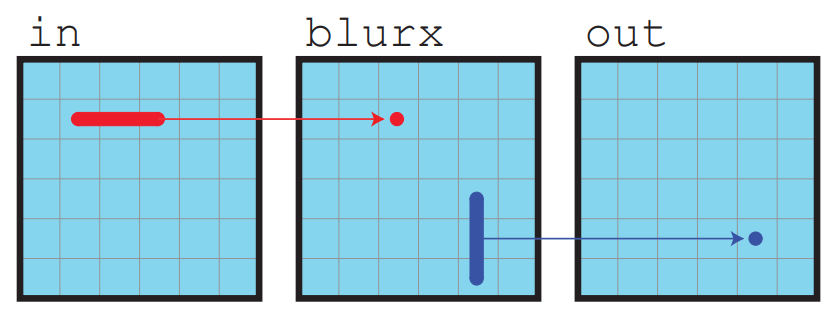
\includegraphics[width=3cm]{img/halide-breadth-first.png}
          \begin{itemize}
            \item[\xmark\xmark] Producer-consumer locality
            \item[\cmark\cmark] Parallelization
            \item[\cmark\cmark] Recomputation
          \end{itemize}
        \end{subfigure}
        \begin{subfigure}[H]{.31\textwidth}
          \centering
          Total fusion/inline strategy
          \inputminted[tabsize=2,frame=single,rulecolor=gray,fontsize=\fontsize{4.2}{3}]{cpp}{fig/blur_3x3_total_fusion.cpp}
          \vspace{0.3cm}
          \centering
          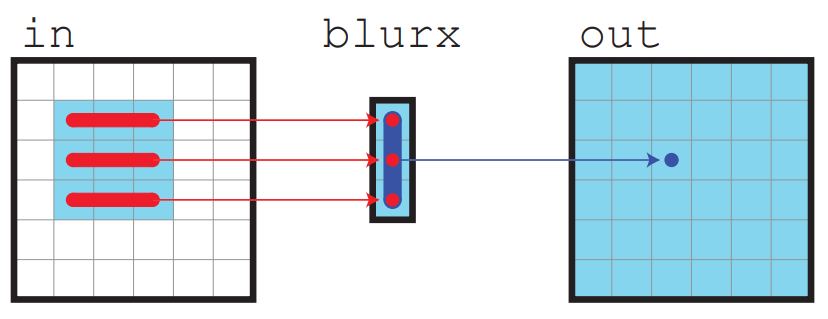
\includegraphics[width=3cm]{img/halide-total-fusion.png}
          \begin{itemize}
            \item[\cmark\cmark] Producer-consumer locality
            \item[\cmark\cmark] Parallelization
            \item[\xmark\xmark] Recomputation
          \end{itemize}
        \end{subfigure}
        \begin{subfigure}[H]{.3475\textwidth}
          \centering
          Sliding window strategy
          \inputminted[tabsize=2,frame=single,rulecolor=gray,fontsize=\fontsize{4.2}{3}]{cpp}{fig/blur_3x3_sliding_window.cpp}
          \centering
          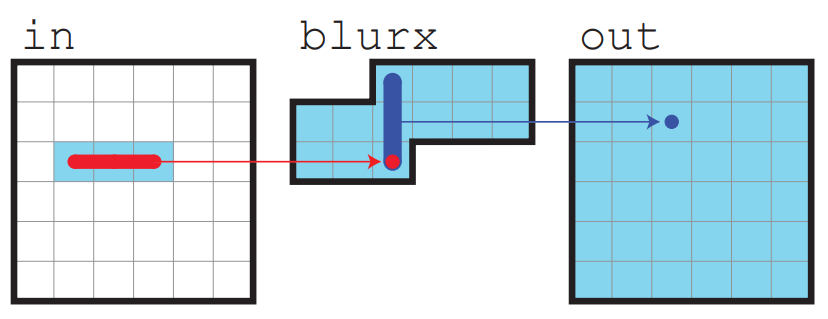
\includegraphics[width=3cm]{img/halide-sliding-window.png}
          \begin{itemize}
            \item[\cmark] Producer-consumer locality
            \item[\xmark\xmark] Parallelization
            \item[\cmark\cmark] Recomputation
          \end{itemize}
        \end{subfigure}
      \end{minipage}
    }
    \centering
    \unskip
    \vspace{0.3cm}
    \begin{tikzpicture}
      \coordinate (a) at (0cm,0cm);
      \coordinate (b) at (1.5cm,0);
      \coordinate (c) at (60:1.5cm);
      %
      \draw[color=black, fill=gray!40] (a) -- (b) -- (c) -- cycle;
      %
      \node[right = 0.1cm of b] {redundant work};
      \node[left = 0.1cm of a] {locality};
      \node[above = 0.1cm of c] {parallelism};
      \node[align=center] at (0.75cm, 0.4cm) {\tiny tradeoff\\\tiny space};
    \end{tikzpicture}
  \end{figure}
\end{frame}

\begin{frame}[fragile]{Scheduling trade-offs (2)}
  \fontsize{6pt}{7.2}\selectfont
  \vspace{0.25cm}
  \begin{figure}[H]
    \makebox[\linewidth]{
      \begin{minipage}{\textwidth}
        \centering
        \begin{subfigure}[H]{.45\textwidth}
          \centering
          Tiling strategy
          \inputminted[tabsize=2,frame=single,rulecolor=gray,fontsize=\fontsize{4.2}{3}]{cpp}{fig/blur_3x3_tiling.cpp}
          \centering
          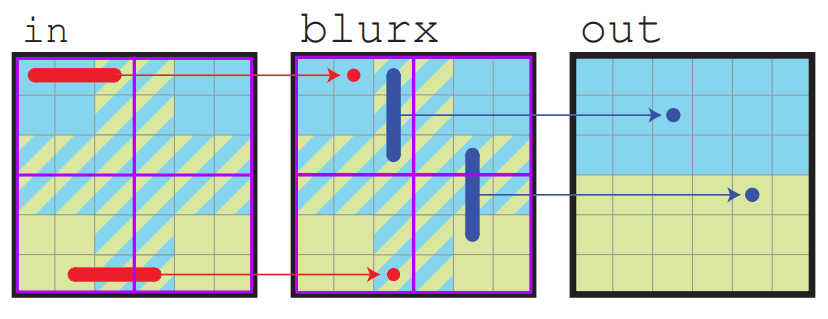
\includegraphics[width=3cm]{img/halide-tiling.png}
          \begin{itemize}
            \item[\cmark] Producer-consumer locality
            \item[\cmark\cmark] Parallelization
            \item[\xmark] Recomputation
          \end{itemize}
        \end{subfigure}
        \begin{subfigure}[H]{.45\textwidth}
          \centering
          Sliding window within tiling strategy
          \inputminted[tabsize=2,frame=single,rulecolor=gray,fontsize=\fontsize{4.2}{3}]{cpp}{fig/blur_3x3_sliding_window_tiling.cpp}
          \vspace{0.4cm}
          \centering
          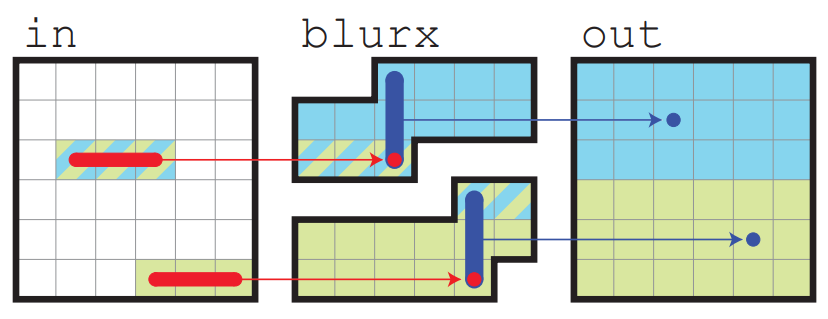
\includegraphics[width=3cm]{img/halide-sliding-window-tiling.png}
          \begin{itemize}
            \item[\cmark] Producer-consumer locality
            \item[\cmark] Parallelization
            \item[\cmark] Recomputation
          \end{itemize}
        \end{subfigure}
      \end{minipage}
    }
  \end{figure}
  \vspace{0.75cm}
  \metroset{block=fill}
  \begin{exampleblock}{Note}
    The best scheduling choice differs depending on each target architecture and the computational characteristics of the image pipeline stages.
  \end{exampleblock}
\end{frame}

\begin{frame}{Halide scheduling example}
  \fontsize{6pt}{7.2}\selectfont
  \begin{enumerate}
    \item Function's \textit{domain} is \textit{tiled} into $64\times64$-sized tiles
    \item Outer two loops of \textit{tiling} are \textit{fused} together into a single loop (\code{tile_index})
    \item \textit{Fused} loop is \textit{parallelized}
    \item Each \textit{tile} is \textit{tiled} again with $4\times2$-sized sub-tiles
    \item Sub-tile innermost $x$-loop (\code{x_vectors}) is \textit{vectorized} with the same factor as \code{x_vectors} ($4$): no iterations will be performed at this nesting level, the whole loop will be vectorized
    \item Sub-tile $y$-loop (\code{y_pairs}) is fully \textit{unrolled} with a factor matching the sub-tile vertical size ($2$), therefore eliminating the sub-tile inner loops in favor of \textit{unrolling} and \textit{vectorization}
  \end{enumerate}

  \begin{figure}[H]
    \begin{minipage}{0.6\textwidth}
      \centering
      \inputminted[tabsize=2,frame=single,rulecolor=gray,fontsize=\fontsize{5}{5}]{cpp}{fig/halide_scheduling_example.cpp}
    \end{minipage}
  \end{figure}
\end{frame}

\begin{frame}{Halide compilation flow}
  \fontsize{6pt}{7.2}\selectfont
  \begin{enumerate}
    \item \textbf{Lowering and loop synthesis}: given the \textit{schedule}, it generates the loop nests and allocations required to evaluate the pipeline, beginning from the output.
    \item \textbf{Bounds inference}: recursively back from the output and using interval analysis, for each function, it evaluates the bounds of the dimensions based on the bounds required by its caller and the indices it is called with.
    \item \textbf{Sliding window optimization and storage folding}: traverses the loop nests seeking opportunities for sliding window optimizations (when the results of a function are to be stored by a serial loop at a higher loop nesting level than its computation).
    \item \textbf{Flattening}: multi-dimensional loads, stores, and allocations are flattened into their linear single-dimensional equivalent.
    \item \textbf{Vectorization and unrolling}: converts loops that were scheduled as vectorized or unrolled into the corresponding loops. During vectorization, occurrences of a loop index are replaced with a special value $ramp(n)$ which represents the vector $[0, 1, \ldots, n-1]$.
    \item \textbf{Back-end code generation}: low-level optimizations are performed and machine code is emitted for the resulting pipeline. After running constant-folding and dead-code elimination passes, the Halide IR is ready to be lowered with a \code{CodeGen} backend. The primary backends use LLVM for code generation.
  \end{enumerate}

  \begin{figure}[H]
    \centering
    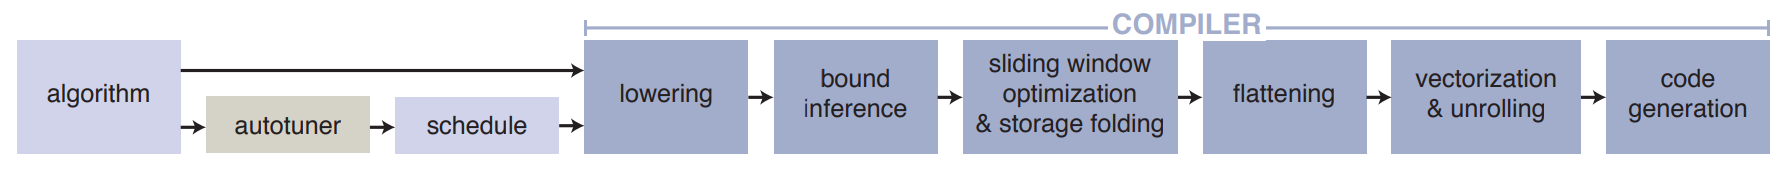
\includegraphics[width=\textwidth]{img/halide-compiler-flow.png}
  \end{figure}

\end{frame}

\begin{frame}{Halide IR}
  \begin{itemize}
    \item Halide IR nodes have an explicit type described by \codecpp{enum IRNodeType}. Examples:
          \begin{itemize}
            \item \codecpp{IntImm} to create integer immediates
            \item \code{Add} to represent additions
            \item \codecpp{Store} and \code{Load} to perform memory accesses
          \end{itemize}
    \item \codecpp{struct IRNode}: \codecpp{IRNodeType} + reference count. Virtual method \codecpp{accept} to implement the \textbf{visitor pattern}.
    \item Two kinds of nodes, analogously to C:
          \begin{itemize}
            \item \textbf{Expressions} (\codecpp{ExprNode}): represent some value and have some type (e.g. \codecpp{x + 3})
            \item \textbf{Statements} (\codecpp{StmtNode}): side-effecting pieces of code that do not represent a value (e.g. \codecpp{assert(x > 3)}).
          \end{itemize}
    \item Type system: signed and unsigned ints, IEEE fp numbers, opaque pointers (like \codecpp{void *}) and \code{bfloat}
  \end{itemize}
  \vspace*{0.1cm}
  \begin{figure}[H]
    \makebox[\linewidth]{
      \begin{minipage}[H]{\textwidth}
        \centering
        \begin{subfigure}[t]{.45\textwidth}
          \centering
          \codecpp{IntImm} node definition
          \inputminted[tabsize=2,frame=single,rulecolor=gray,fontsize=\fontsize{4.5}{4}]{cpp}{fig/halide_IntImm_node.cpp}
        \end{subfigure}
        \begin{subfigure}[t]{.475\textwidth}
          \centering
          \codecpp{IfThenElse} node definition
          \inputminted[tabsize=2,frame=single,rulecolor=gray,fontsize=\fontsize{4.5}{4}]{cpp}{fig/halide_IfThenElse_node.cpp}
          \vspace{0.4cm}
        \end{subfigure}
      \end{minipage}
    }
  \end{figure}
\end{frame}

\section{MLIR}

\begin{frame}{\raisebox{-0.25\height}{
\includegraphics[height=0.5cm]{img/mlir-identity-09.png}}}
  \begin{itemize}
    \item Multi-Level Intermediate Representation (MLIR): open-source compiler infrastructure project; provides common IR to represent \textbf{multiple levels of abstractions} maintaining a \textbf{unified interface}.
    \item Under LLVM's umbrella.
    \item Address challenges in building compilers and optimizing code generation for modern high-performance computing and machine-learning applications.
          \begin{itemize}
            \item Many compilation and system design problems are better modeled at a \textbf{higher-} or \textbf{lower-level abstraction}. Languages that use LLVM end up developing their IR to solve domain-specific problems. ML frameworks also use domain-specific abstractions (\textquote{ML graphs}).
            \item Makes it \textbf{easy} to define and \textbf{introduce new abstraction levels} and provides the infrastructure to use them to solve common compiler engineering problems.
          \end{itemize}
    \item MLIR infrastructure provides:
          \begin{enumerate}
            \item Standardized Static Single Assignment (\textbf{SSA})-based IR data structures,
            \item Declarative system for defining IR \textbf{dialects}, and
            \item Wide range of common infrastructure: documentation, parsing and printing logic, multithreaded compilation support, \textbf{pass management}, etc.
          \end{enumerate}
  \end{itemize}
\end{frame}

\begin{frame}{\raisebox{-0.25\height}{
\includegraphics[height=0.5cm]{img/mlir-identity-09.png}} Dialects}
  \begin{itemize}
    \item \textbf{Dialect}: collection of related \textbf{operations}, \textbf{attributes} and \textbf{types} used to represent a particular domain.
          \begin{itemize}
            \item \textit{Attributes}: mechanism for specifying constant data on operations in places where a variable is never allowed (such as the comparison predicate of a \code{cmpi} operation).
          \end{itemize}
    \item MLIR allows for multiple dialects (even those outside of the main code tree) to \textbf{co-exist} together within one \textit{module}. Dialects are produced and consumed by certain \textbf{\textit{passes}}.
    \item Examples:
          \begin{itemize}
            \item \textbf{\textit{Arith}}: arithmetic dialect, holds basic integer and floating point mathematical operations which include: unary, binary, and ternary arithmetic ops, bitwise and shift ops, cast ops, and compare ops. Operations in this dialect also accept vectors and tensors of integers or floats.
            \item \textbf{\textit{Func}}: creation of high-level function abstractions and function calls.
            \item \textbf{\textit{Memref}}: memory reference, provides a collection of operations and types focused on representing and manipulating multi-dimensional arrays, or tensors, in memory.
            \item \textbf{\textit{SCF}}: structured control flow, which includes operations such as loops and conditionals.
            \item \textbf{\textit{Vector}}: supports multi-dimensional vector types and custom operations on them.
            \item \textbf{\textit{Affine}}: affine expressions and affine loops that allows polyhedral model compilation, analysis and optimizations.
          \end{itemize}
  \end{itemize}
\end{frame}

\begin{frame}{\raisebox{-0.25\height}{
\includegraphics[height=0.5cm]{img/mlir-identity-09.png}} IR}
  \begin{itemize}
    \item IR is \textbf{generic} enough to represent ASTs in a language frontend, generated instructions in a target-specific backend, HLS constructs, circuits (CIRCT), etc.
    \item IR is based on a graph-like data structure:
          \begin{itemize}
            \item Nodes: \textbf{\textit{Operations}}
            \item Edges: \textbf{\textit{Values}}
          \end{itemize}
          Each \textit{Value} is the result of exactly one \textit{Operation} or \textbf{\textit{Block Argument}} and has a \textbf{\textit{Value Type}} defined by the type system.
    \item Three forms: human-readable (\code{.mlir}), in-memory and serialized.
  \end{itemize}
  \begin{figure}[H]
    \centering
    \begin{minipage}{0.475\textwidth}
      \inputminted[tabsize=2,frame=single,rulecolor=gray,fontsize=\fontsize{6}{6}]{text}{fig/mlir_ir_example.mlir}
    \end{minipage}
  \end{figure}
\end{frame}

\section{CIRCT}

\begin{frame}{\raisebox{-0.25\height}{
\includegraphics[height=0.5cm]{img/circt-logo.png}} CIRCT}
  \begin{itemize}
    \item \textbf{C}ircuit \textbf{IR} \textbf{C}ompilers and \textbf{T}ools (CIRCT): project built \textbf{on top of MLIR}. Provides a set of tools and libraries to help with the \textbf{design} and verification of \textbf{digital circuits}.
    \item Adds new \textbf{hardware-oriented dialects} such as:
          \begin{itemize}
            \item \textit{\textbf{\code{hw}}}: generic HW dialect where other dialect operations are instantiated.
            \item \textit{\textbf{\code{comb}}}: models digital combinational logic.
            \item \textit{\textbf{\code{seq}}}: models digital sequential logic.
            \item \textit{\textbf{\code{fsm}}}: models finite-state machines.
            \item \textit{\textbf{\code{sv}}}: represents various SystemVerilog-specific constructs.
            \item \textit{\textbf{\code{calyx}}}: represents Calyx IR types and operations.
          \end{itemize}
    \item Provides a static scheduling infrastructure:
          \begin{itemize}
            \item A \texit{problem} is created from the IR (such as \textit{ModuloProblem}).
            \item A \textit{scheduler} solves the problem (list scheduler, LP-based schedulers, etc).
            \item \code{AffineToLoopSchedule} pass uses Calyx operator library for operation latencies and lowers to \code{LoopSchedule} dialect.
          \end{itemize}
    \item \codecpp{circt::createExportVerilogPass()} takes IR and emits SystemVerilog code.
          \begin{itemize}
            \item Style and options controlled by \codecpp{struct circt::LoweringOptions}.
          \end{itemize}
    \item Under LLVM's umbrella.
    \item SiFive contributing to CIRCT (order of magnitude faster than the current Chisel compiler).
  \end{itemize}
\end{frame}

\begin{frame}{\raisebox{-0.25\height}{
\includegraphics[height=0.5cm]{img/circt-logo.png}} CIRCT Dialects and conversion passes}
  \begin{figure}[H]
    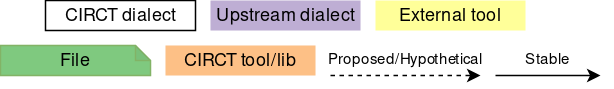
\includegraphics[width=4.1cm,left]{img/circt-dialectlegend.png}
  \end{figure}
  \begin{figure}[H]
    \centering
    \vspace*{-1.1cm}
    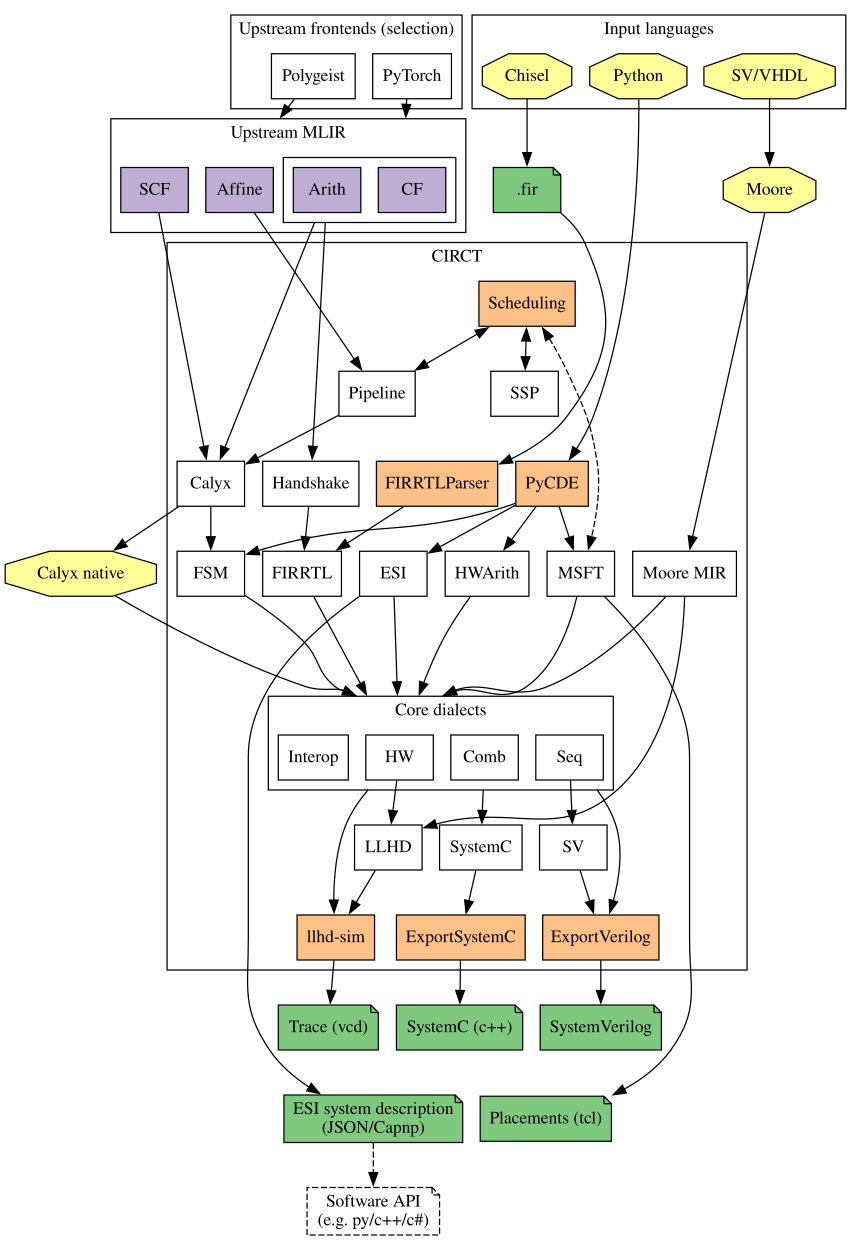
\includegraphics[height=8.1cm]{img/circt-dialects.png}
  \end{figure}
\end{frame}

\section{Calyx}

\begin{frame}{\raisebox{-0.25\height}{
\includegraphics[height=0.5cm]{img/calyx-logo-text.png}}}
  \begin{itemize}
    \item TODO
  \end{itemize}
\end{frame}

\end{document}
